\documentclass[a4paper]{article}

\usepackage{isapreamble}

\title{\huge \textbf{MA E\(\chi\) 02}}
\author{
  isagila
  \and
  \href{https://t.me/pochtineploho}{@pochtineploho}
  \and
  \href{https://t.me/DUBSTEPHAVEGUN}{@DUBSTEPHAVEGUN}
}
\date{Собрано {\ddmmyyyydate\today} в \currenttime}
\titlepic{
\includegraphics[width = \textwidth]{misc/title.png}}

\begin{document}

%% Отступы перед/после формул
\setlength{\abovedisplayskip}{-5pt}
\setlength{\abovedisplayshortskip}{0pt}
\setlength{\belowdisplayskip}{0pt}
\setlength{\belowdisplayshortskip}{0pt}

\clearpage
\maketitle
\thispagestyle{empty}
\newpage
\setcounter{page}{2}
\begin{figure}[h]
  \center{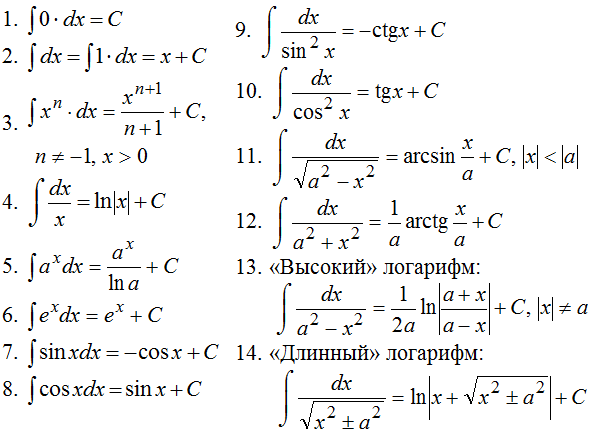
\includegraphics[width=\textwidth]{misc/table_of_integrals.png}}
\end{figure}
\pagebreak
\tableofcontents

\newpage
\section{Интегрирование функции одной переменной}

\begin{questions}
  \foreach \idx in {01, ..., 24} {
    \input{./SI/\twodigits\idx}
  }
\end{questions}

\newpage
\section{Интегрирование функции нескольких переменных}

\begin{questions}
  \foreach \idx in {01, ..., 23} {
    \input{./MI/\twodigits\idx}
  }
\end{questions}

\end{document}